\documentclass[12pt]{beamer}
\usetheme{Boadilla}

\usepackage[utf8]{inputenc}
\usepackage[T1]{fontenc}
\usepackage[francais]{babel}
\usepackage{amsmath}
\usepackage{amsfonts}
\usepackage{amssymb}
\usepackage{graphicx}
\setbeamertemplate{enumerate items}[square]

\author{Thomas \textsc{Citharel}}
\title{Soutenance de stage}
\subtitle{Développement et mise en place d'une application de gestion d'agendas}
\logo{}
\institute{IUT d'Orléans}
\date{31 août 2016}
\subject{sujet}
\setbeamercovered{transparent}
\setbeamertemplate{navigation symbols}{}

\begin{document}
	\maketitle
	
	\begin{frame}
		\frametitle{Sommaire}
		\tableofcontents
	\end{frame}
	\section{Présentation de la structure}
	\subsection{Historique}
	\begin{frame}
		\frametitle{Présentation de la structure}
		
		\begin{minipage}{0.45\textwidth}
			\begin{flushleft}
				\begin{itemize}
					\item Organisation à but non lucratif (Association Loi 1901)
					\item Promotion du \textbf{logiciel libre}, de la \textbf{culture libre} et des \textbf{services libres}
					\item Fondée en \textbf{2004} à partir d'un site web datant de 2001.
				\end{itemize}
			\end{flushleft}
		\end{minipage}
		\begin{minipage}{0.45\textwidth}
			\begin{flushright}
				\begin{figure}
					\centering
					
\includegraphics[width=0.7\linewidth]{images/Framasoft-Logo}
					\caption{Logo de Framasoft}
					\label{fig:framasoft-logo}
				\end{figure}
			\end{flushright}
		\end{minipage}
	\end{frame}
	\begin{frame}
		\frametitle{Présentation de la structure}
		Différents projets :
		\begin{itemize}
			\visible<1->{\item \textbf{2001} - Annuaire de logiciels libres}
			\visible<2->{\item \textbf{2004} - Diffusion de logiciels libres par la Framakey puis les Framadvd}
			\visible<3->{\item \textbf{2006} - Publication d'ouvrages sous licences libres (Framabook)}
			\visible<4->{\item \textbf{2011} - Mise en place des premiers services libres (Framapad, Framadate, ...)}
		\end{itemize}
	\end{frame}
	\begin{frame}
		\frametitle{Présentation de la structure}
		\begin{minipage}{0.45\textwidth}
			\begin{flushleft}
				Montrer au grand public les alternatives qui existent face aux services non respectueux de la vie privée (\textit{GAFAM}).
			\end{flushleft}
		\end{minipage}
		\begin{minipage}{0.45\textwidth}
			\begin{flushright}
				\begin{figure}[ht]
					\centering
					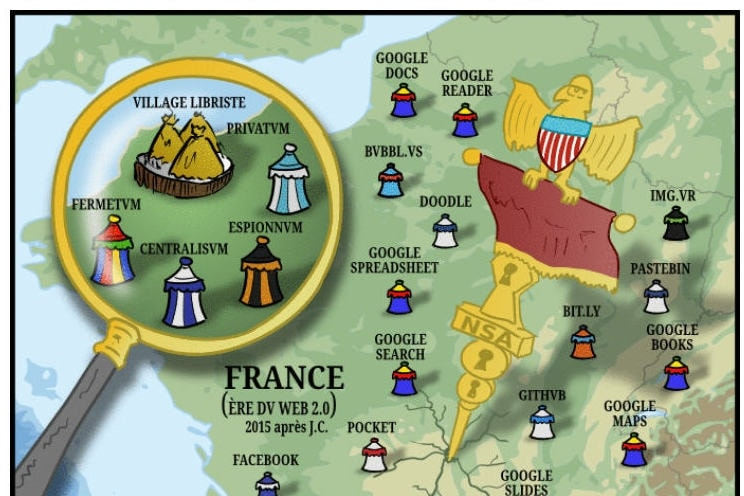
\includegraphics[width=0.9\linewidth]{images/degooglisons-internet}
					\caption{Carte de la campagne Dégooglisons}
					\label{fig:degooglisons-carte}
				\end{figure}
			\end{flushright}
		\end{minipage}
		
		\subsection{Liste des services}
		
		\centering
		\begin{tabular}{|l|l|}
			\hline
			\emph{Service en ligne} & \emph{Alternative} \\
			\hline
			Google Docs & Framapad \\
			\hline
			Google Spreadsheet & Framacalc \\
			\hline
			Doodle & Framadate \\
			\hline
			Facebook & Framasphère \\
			\hline
			Pocket & Framabag \\
			\hline
		\end{tabular}
	\end{frame}
	\section{Présentation du projet}
	\begin{frame}
		\frametitle{Présentation du projet}
		\subsection{Alternative à Google Agenda}
		\begin{figure}
				\centering
				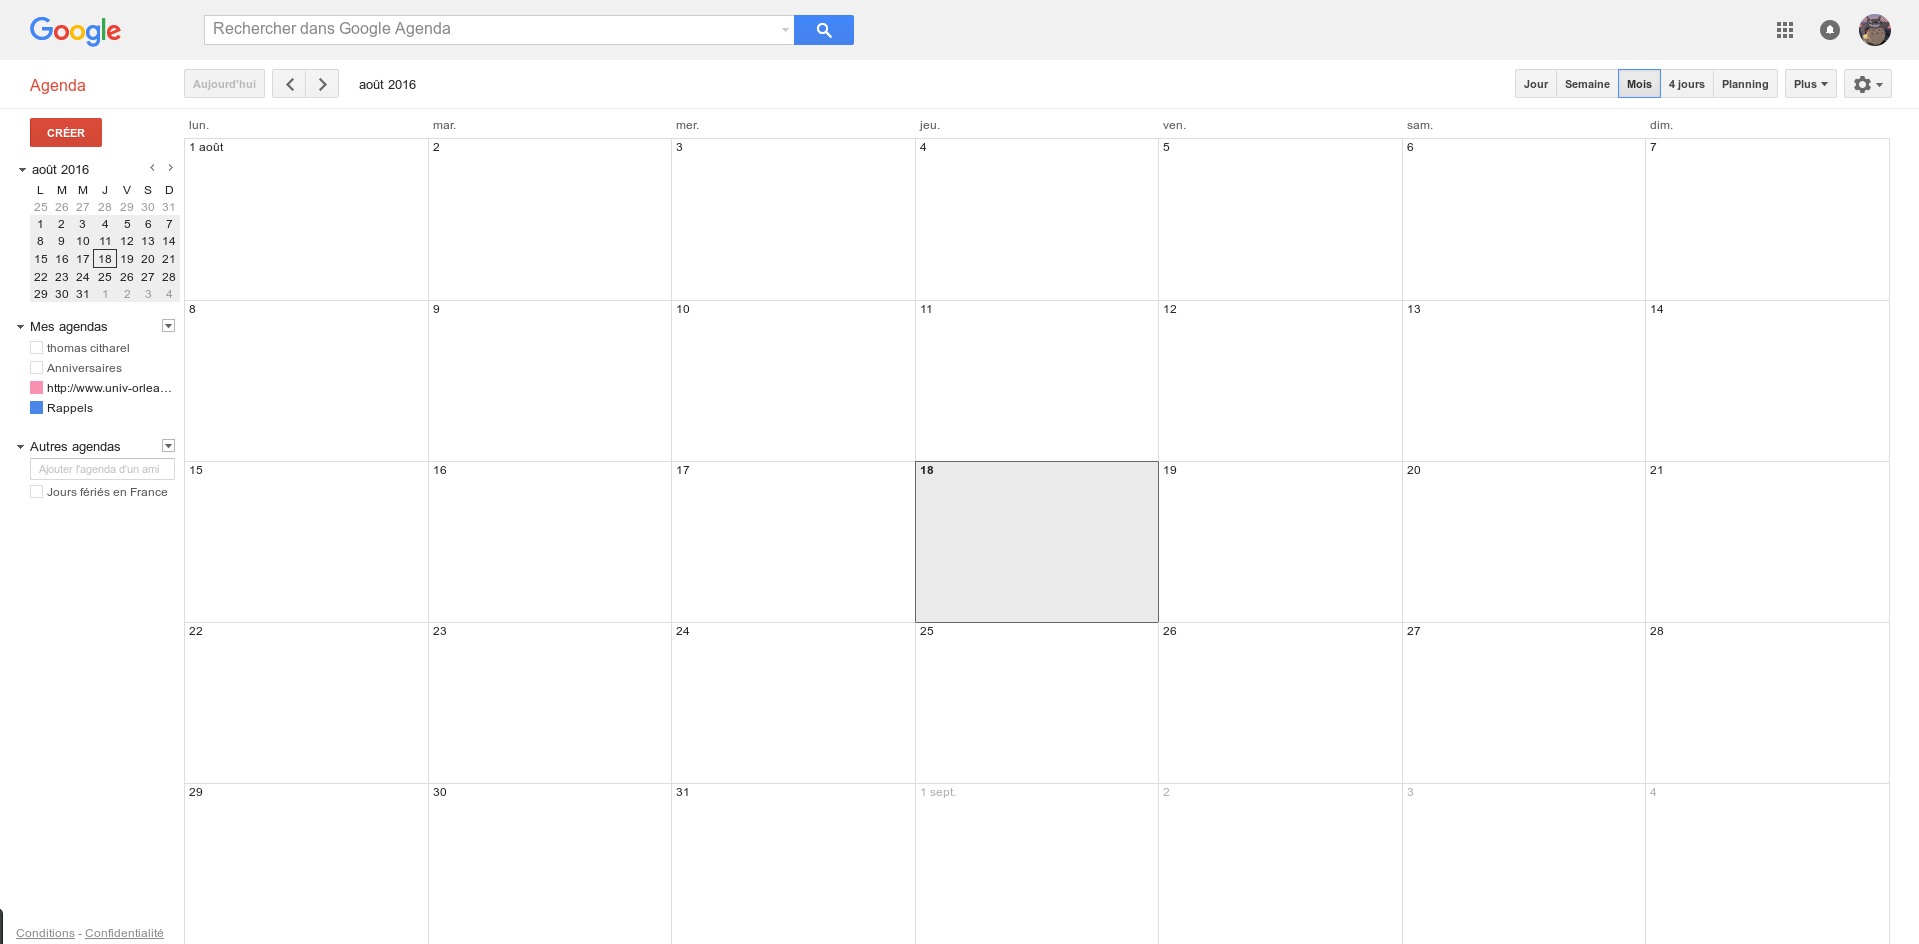
\includegraphics[width=1\linewidth]{images/google-agenda-interface-actuelle}
				\caption{Aperçu de Google Agenda}
				\label{fig:google-agenda-interface-actuelle}
			\end{figure}
		\end{frame}
		\begin{frame}
			\frametitle{Présentation du projet}
			Choix de l'application sur laquelle se baser.
			\begin{itemize}
				\visible<1->{\item Nécessité d'avoir un bon nombre de fonctionnalités déjà existantes}
				\visible<2->{\item Interface utilisateur intuitive et moderne}
				\visible<3->{\item Logiciel pas trop vieux afin d'éviter une dette technique}
			\end{itemize}
		\end{frame}
		\begin{frame}
		\frametitle{Présentation du projet}
		\visible<1->{Solution basée sur \textbf{ownCloud} et son application Calendar.}
		\begin{itemize}
			\visible<2->{\item Créée en \textbf{2008}}
			\visible<3->{\item Écrite en \textbf{PHP}}
			\visible<4->{\item Fonctionnement autour d'un cœur et d'un ensemble d'applications}
		\end{itemize}
		\end{frame}
		\subsection{L'application existante}
		\begin{frame}
		\frametitle{Présentation du projet}
			Fonctionnalités existantes
			\begin{enumerate}
				\visible<1->{\item Gestion de la liste d'agendas}
				\visible<2->{\item Gestion d'événements}
				\visible<3->{\item Partage d'événements}
				\visible<4->{\item Synchronisation avec applications clientes}
				\visible<5->{\item Import/Export d'agendas}
			\end{enumerate}
	\end{frame}
	\section{Objectifs du stage}
	\begin{frame}
		\frametitle{Objectifs du stage}
		\begin{enumerate}
		\visible<1->{\item Ajout de fonctionnalités}
		\begin{enumerate}
			\visible<2->{\item Publication d'un calendrier (partage d'un calendrier par un lien public)}
			\visible<3->{\item Abonnement à des calendriers (ajout de sources en ligne en lecture seule)}
		\end{enumerate}
		\visible<3->{\item Mise en place du service}
		\visible<4->{\item Rédaction de la documentation}
	\end{enumerate}
	\end{frame}
	\section{Réalisation du projet}
	\begin{frame}
		\frametitle{Réalisation du projet}
		\begin{itemize}
			\visible<1->{\item Utilisation de l'éditeur Atom, de PHP et de SQLite.}
			\visible<2->{\item Mise en place sur une machine virtuelle avec un nom de domaine pour effectuer des tests utilisateur}
			\visible<3->{\item Tests pratiques de la synchronisation avec des applications clientes}
		\end{itemize}
	\end{frame}
	\section{Bilan}
	\subsection{Bilan technique}
	\begin{frame}
		\frametitle{Bilan}
		Bilan technique :
		\begin{itemize}
			\item Apprentissage de certains \textit{design patterns} en PHP.
			\item Bonne introduction au framework AngularJS
			\item Utilisation avancée de Git
			\item Code intégré \textit{upstream} : retours sur la qualité du code
		\end{itemize}
	\end{frame}
	\subsection{Bilan humain}
	\begin{frame}
		\frametitle{Bilan}
		Bilan humain:
		\begin{itemize}
			\item Travail à distance des autres développeurs de l'application (IRC, Github)
			\item Confirmation de mon objectif professionnel qui s'est traduit par une embauche dans l'association
		\end{itemize}
	\end{frame}
	\begin{frame}
		\frametitle{Questions}
		\centering \LARGE Questions
	\end{frame}
\end{document}